\documentclass[11pt,a4paper]{jsarticle}
%

\usepackage{amsmath,amssymb}
\usepackage{bm}
\usepackage[dvipdfmx]{color}
\usepackage[dvipdfmx]{graphicx}
\usepackage{ascmac}
\usepackage{listings, jlisting}
\lstset{%
  basicstyle={\small},%
  identifierstyle={\small},%
  commentstyle={\small\itshape},%
  keywordstyle={\small\bfseries},%
  ndkeywordstyle={\small},%
  stringstyle={\small\ttfamily},
  breaklines=true,
  columns=[l]{fullflexible},%
  numbers=none,%
  xrightmargin=0zw,%
  xleftmargin=3zw,%
  numberstyle={\scriptsize},%
  stepnumber=1,
  numbersep=1zw,%
  lineskip=-0.5ex%
}


%
\setlength{\textwidth}{\fullwidth}
\setlength{\textheight}{40\baselineskip}
\addtolength{\textheight}{\topskip}
\setlength{\voffset}{-0.2in}
\setlength{\topmargin}{0pt}
\setlength{\headheight}{0pt}
\setlength{\headsep}{0pt}

%
\newcommand{\divergence}{\mathrm{div}\,}  %ダイバージェンス
\newcommand{\grad}{\mathrm{grad}\,}  %グラディエント
\newcommand{\rot}{\mathrm{rot}\,}  %ローテーション
%
\title{チャレンジサイト・メカニックカモノハシ2019\\マイクロマウスシミュレータExercise}
%\author{ER17045 立道壱太郎}
%\date{\today}
\begin{document}
\maketitle
%
%
\section{この資料について}
メカニックカモノハシではマイクロマウス大会に参加することでメンバーの技術向上を図ります。
資料等はgithubに公開しているので、適時ダウンロードしてください。

\begin{lstlisting}[frame=single]
$ git clone https://github.com/platypus5384/micro_mouse.git
\end{lstlisting}

また、PC・Ubuntuの基本操作、vimの基本操作、プログラミング言語の基礎知識(if文・for文・配列等)が
多少(講義を受けた、1周間くらい使ったことがある程度)を想定しています。
最初は復習から始めますが、日常生活でも練習しておいてください。


\section{動作環境について}
\begin{itemize}
\item{} Ubuntu16.04LTS
\item{} ROS Kinetic
\end{itemize}

での動作を前提としています。
Ubuntu18.04LTS等でも問題ないと思いますが、ros関連のパッケージ名が違ってくるので注意(kineticをmelodic等に変えるだけなので簡単)


\section{Exercise}
\subsection{Python簡易入門}
Python2.7での動作を想定しています。以下を実行し、2.7.xxxのような出力になれば問題ありません。
\begin{lstlisting}[frame=single]
$ python -V
2.7.12
\end{lstlisting}

Pythonを学ぶに至っては「Python 入門」等と調べると、
丁寧でわかりやすいサイトが、たくさん多く出てくるので、
このPDFではマイクロマウスシミュレータを触りながらPythonを学ぶ事にします。
以下のサイトを見る事を想定して資料を作っています。
(以降、このサイトを参考サイトと呼びます。ちなみにこのサイトは別に親切な訳では無いです。)
\begin{lstlisting}[frame=single]
http://tohoho-web.com/python/index.html
\end{lstlisting}

\newpage
\subsection{マウスシミュレータを起動しよう}
マウスシミュレータを起動・試運転させましょう。
それぞれ別のタブで実行してください。
\begin{lstlisting}[frame=single]
$ roslaunch micro_mouse start_up.launch
\end{lstlisting}

実行すると、2つのウィンドウが開き、以下の図\ref{mms_startup}のような画面になります。
\begin{figure}[h]
  \begin{center}
    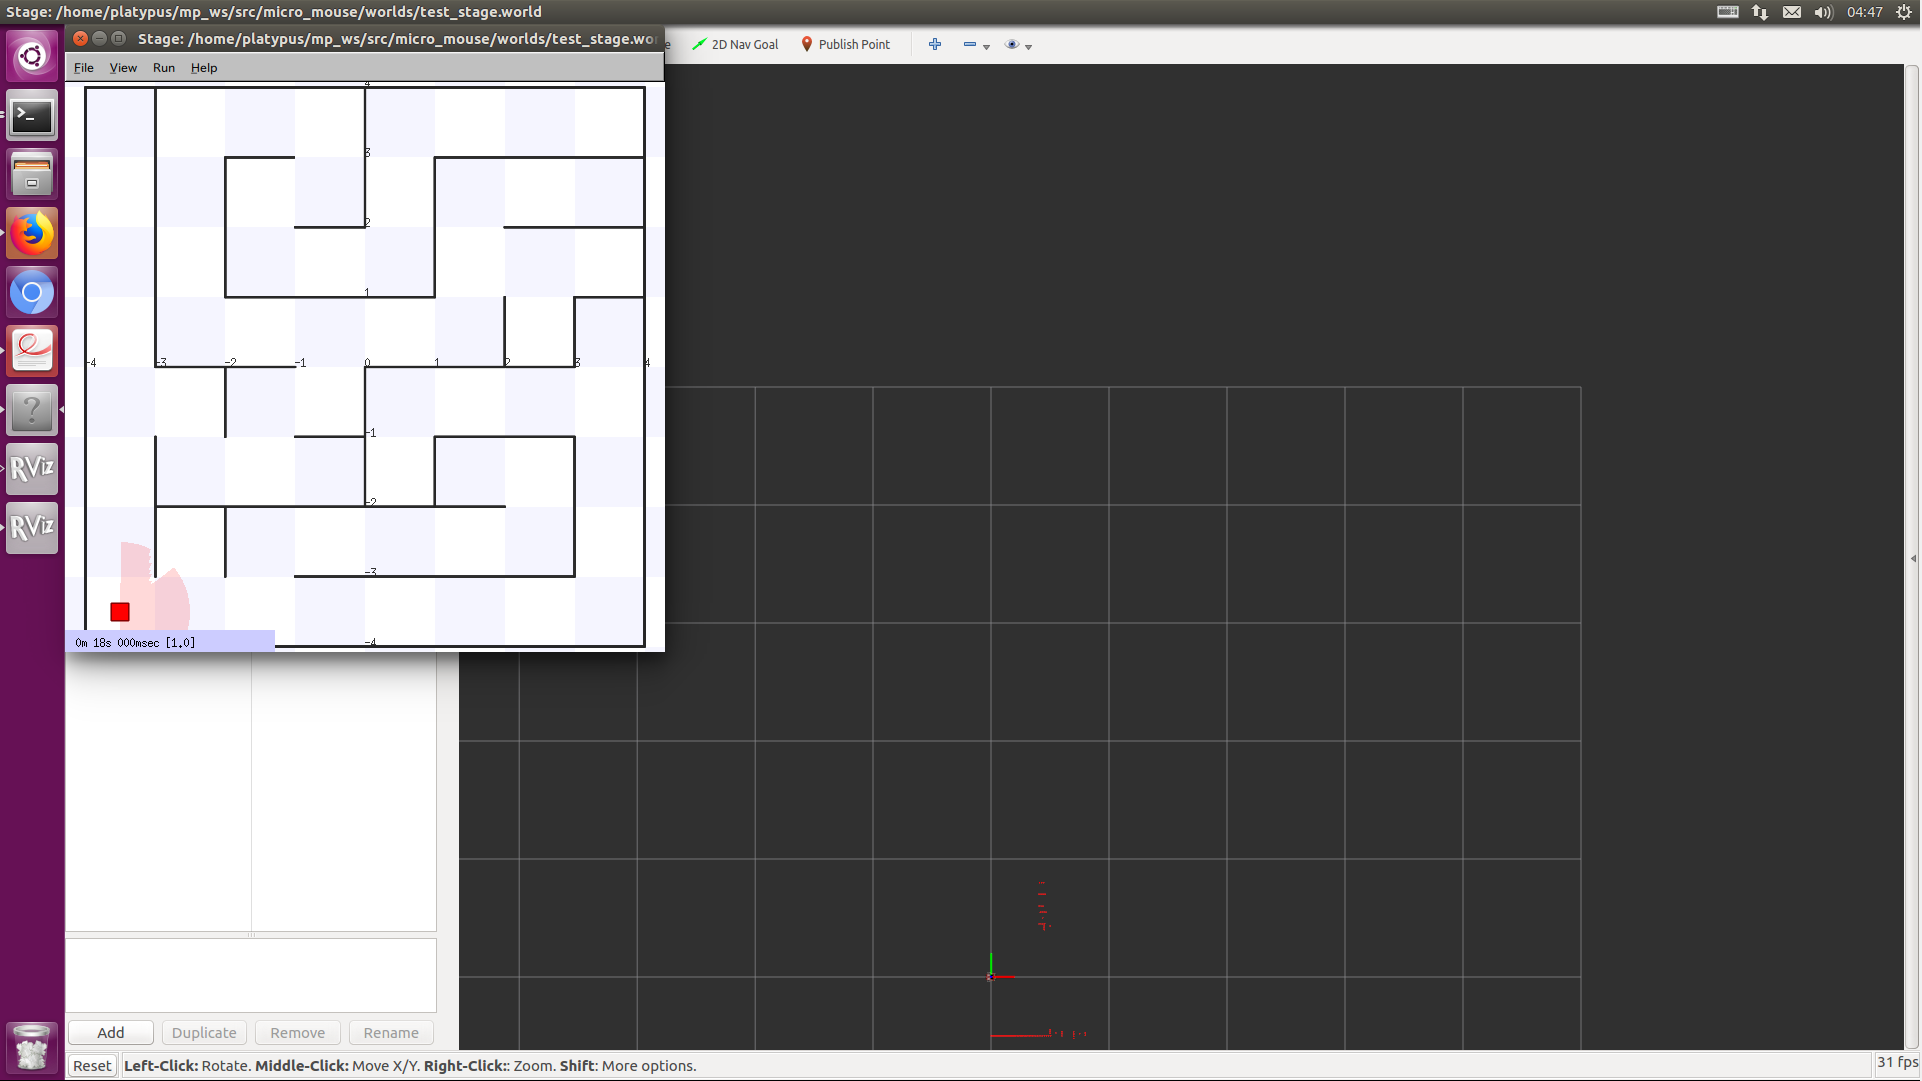
\includegraphics[width=128mm]{./mms_startup.png}
  \end{center}
  \label{mms_startup}
  \caption{マイクロマウスシミュレータを実行した時の様子}
\end{figure}

以下の写真のようなウィンドウはマイクロマウスのシミュレータです。
実際のステージと思って貰って大丈夫です。
\begin{figure}[h]
  \begin{center}
    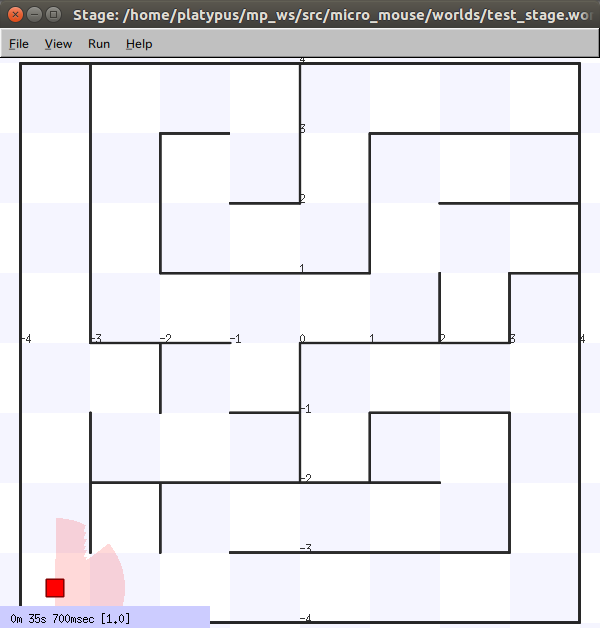
\includegraphics[width=64mm]{./mms_simulator.png}
  \end{center}
  \label{mms_simulator}
  \caption{マイクロマウスシミュレータ}
\end{figure}

以下の写真のようなウィンドウはRvizと呼ばれる、情報を可視化するツールです。ROS標準の物です。
上記のシミュレータに直接書き込むことは出来ないので、こちらに壁や地図等を表示させます。
実際のロボット開発でも使われており、メカニックカモノハシでも多用します。非常に便利なものなので慣れましょう。
\begin{figure}[h]
  \begin{center}
    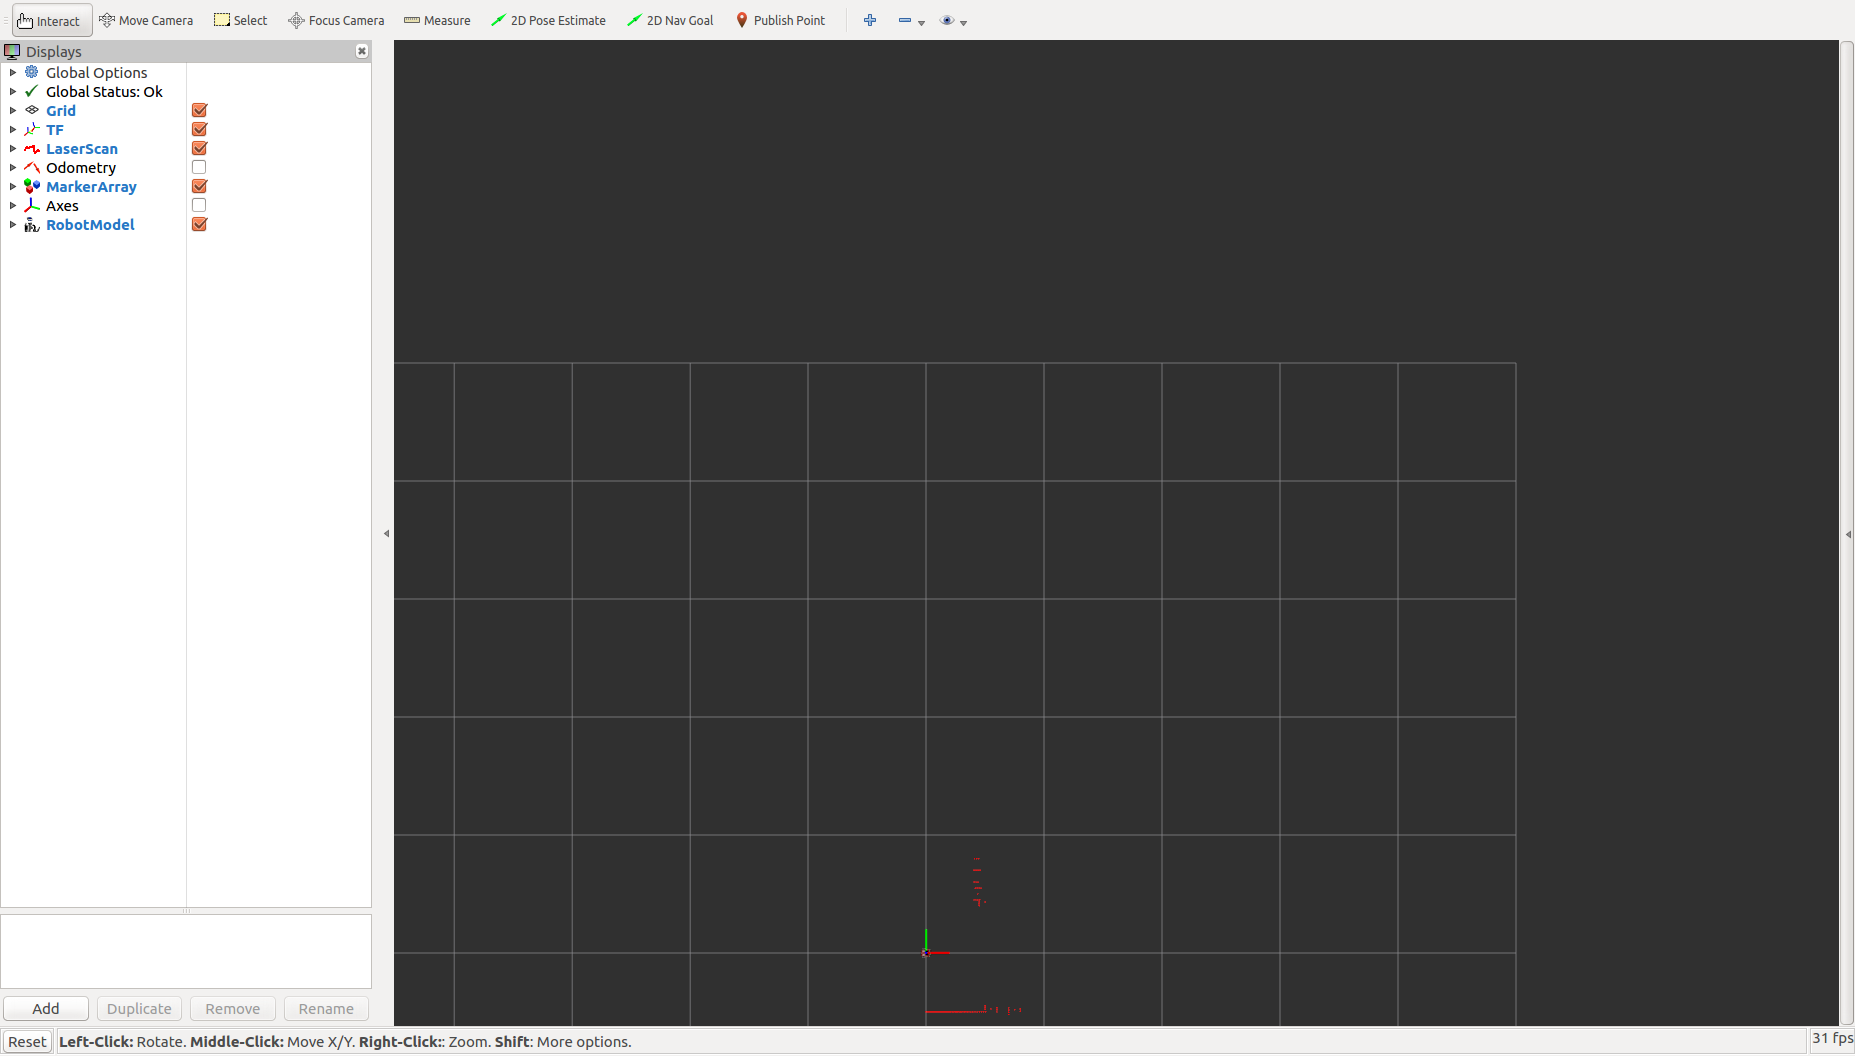
\includegraphics[width=100mm]{./mms_rviz.png}
  \end{center}
  \label{mms_simulator}
  \caption{Rviz}
\end{figure}



\subsection{マウスシミュレータでマウスを動かそう}

試運転に以下を実行してみましょう。拡張左手法のプログラムです。
\begin{lstlisting}[frame=single]
$ rosrun micro_mouse left_hund_ex.py
\end{lstlisting}

実行するとマウスが動き出し、Rvizに壁やタイルが描画されていきます。

ロボットが動き出し、マッピングが始まれば成功です。
しばらく待つと、以下のようになります。
\begin{figure}[h]
  \begin{center}
    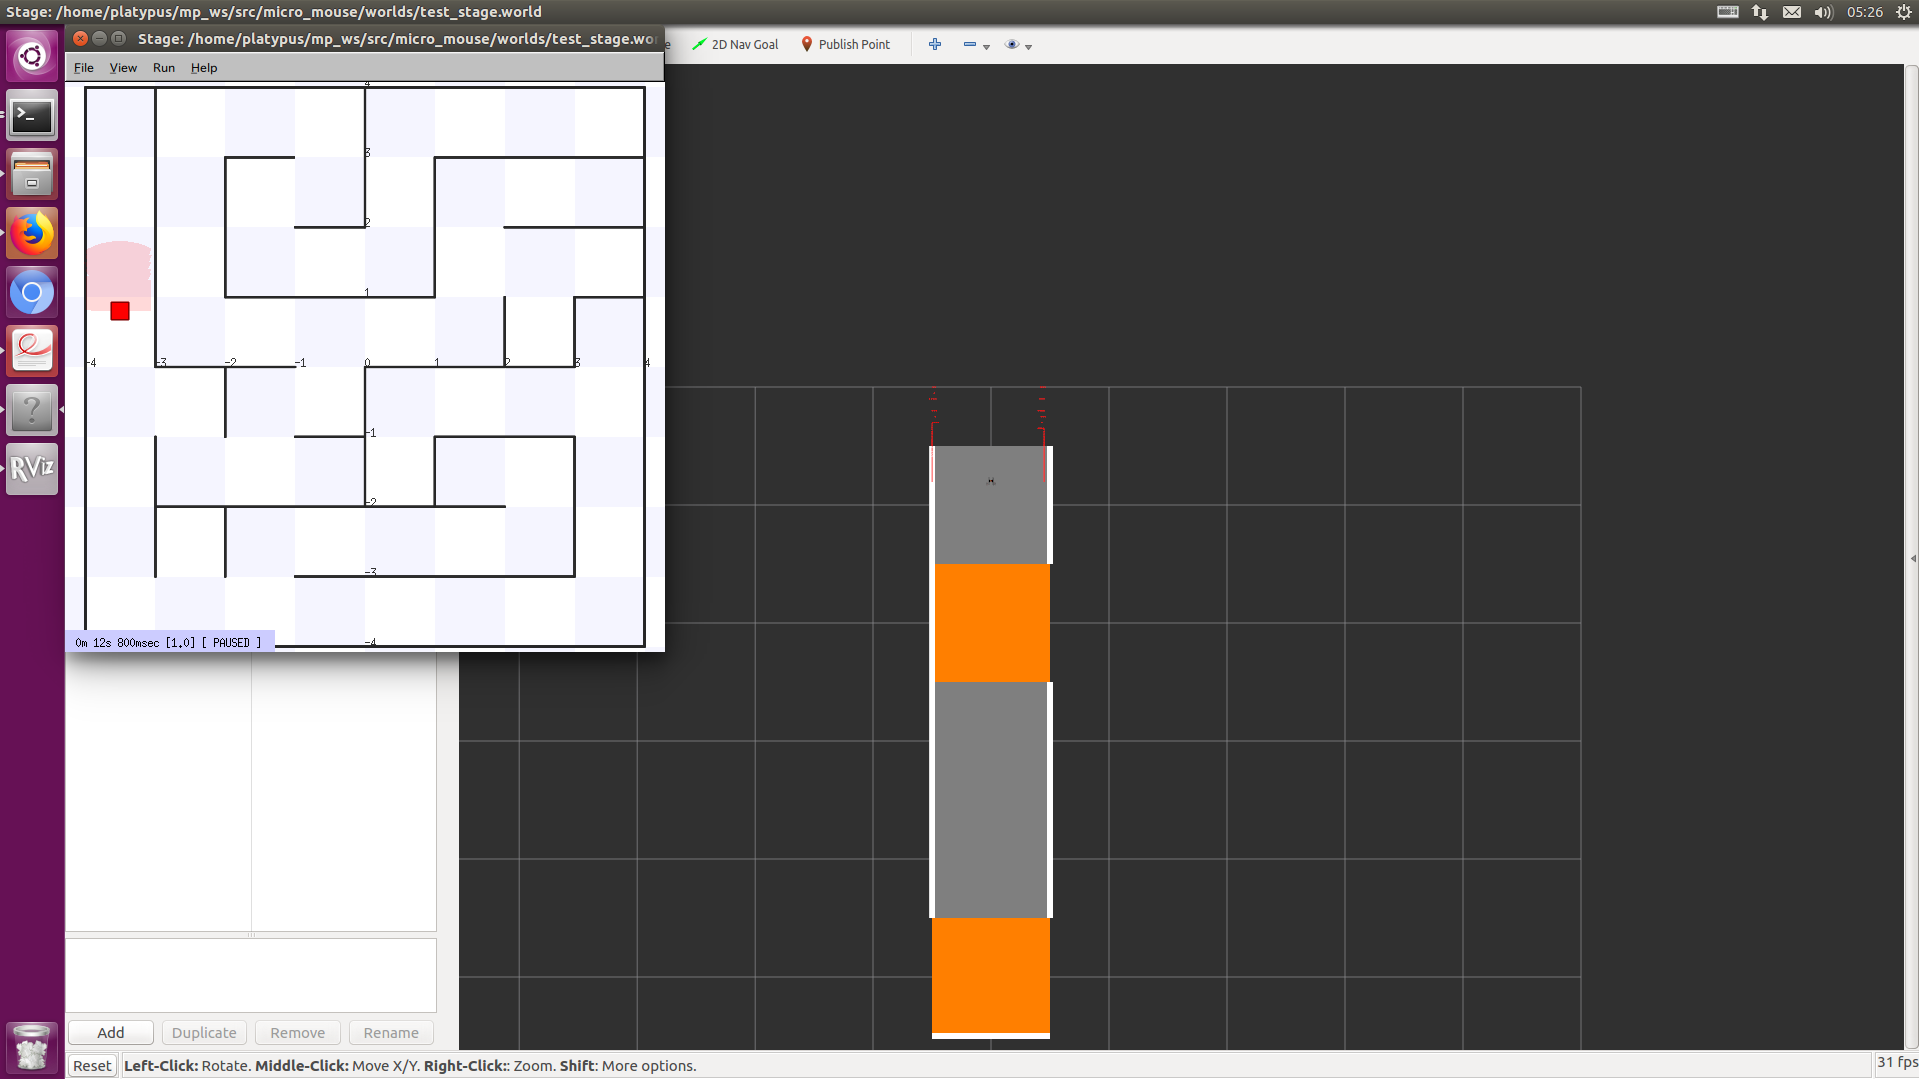
\includegraphics[width=128mm]{./mms_test_pause.png}
  \end{center}
  \label{mms_simulator}
  \caption{left\_hund\_ex.pyを実行した直後}
  \caption{}
  \label{test}
\end{figure}

せっかくなので、シミュレータの時間停止、加速、減速などを試しましょう。
以下を試してみてください。(シミュレータのツールバーに載っています)
\begin{itemize}
\item{ p} 時間停止・開始
\item{ [} 減速
\item{ ]}加速(2倍速以上?にすると脱線します)
\end{itemize}


\subsection{マウスシミュレータをリセットしよう}
まずは、プログラム(rosrun)を中断してください。
中断したら、以下を実行してください。
\begin{lstlisting}[frame=single]
rosservice call /reset_positions
\end{lstlisting}
実行するとマウスが初期位置に戻ります。(Rvizは初期化されませんが問題ありません)

\section{Exercise}
\subsection{Python簡易入門}
簡易的にPython入門しよう。
使用するソースコード等は、\verb|micro_mouse/script/chapter/0|にあります。

\subsection{プログラミング言語の3大要素}
プログラミング言語の3大要素は「順次」、「選択」、「繰り返し」です。
これはどの言語でも共通で、これさえ覚えれば、(労力はかかるが)なんでもできます。\\


3大要素について解説します。

まず、「順次」とは、上から下に順番に実行していくことです。それだけです。\\


次に、「選択」とは「もしAならばBする」という処理です。
例えば、「もし、ジュースが100円以下ならば、1本買う」、「もし、授業日ならば、学校に行く」と言った感じです。\\


最後に、「繰り返し」とは、その名の通り繰り返しを行います。
例えば、私達は「もし、日曜ならば、学校は休み」という選択を毎日やっていますが、
これをプログラムで書く場合は「在学中なら、次の文を繰り返す」「もし、授業日ならば、学校に行く」というように書きます。
\begin{figure}[htbp]
 \begin{minipage}{0.3\hsize}
  \begin{center}
   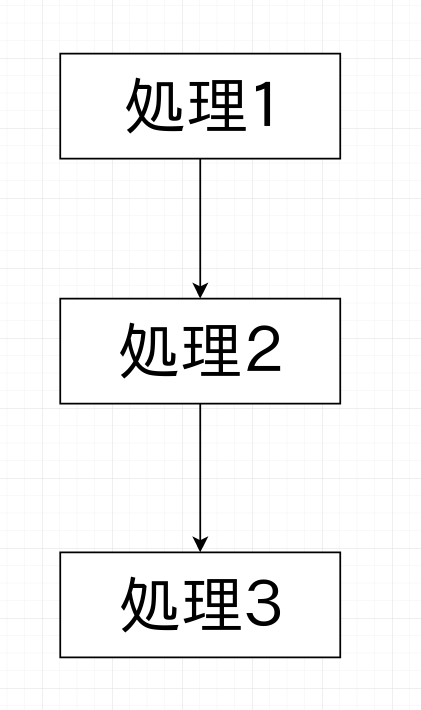
\includegraphics[width=20mm]{./sequential.png}
  \end{center}
  \caption{順次}
 \end{minipage}
 \begin{minipage}{0.3\hsize}
 \begin{center}
  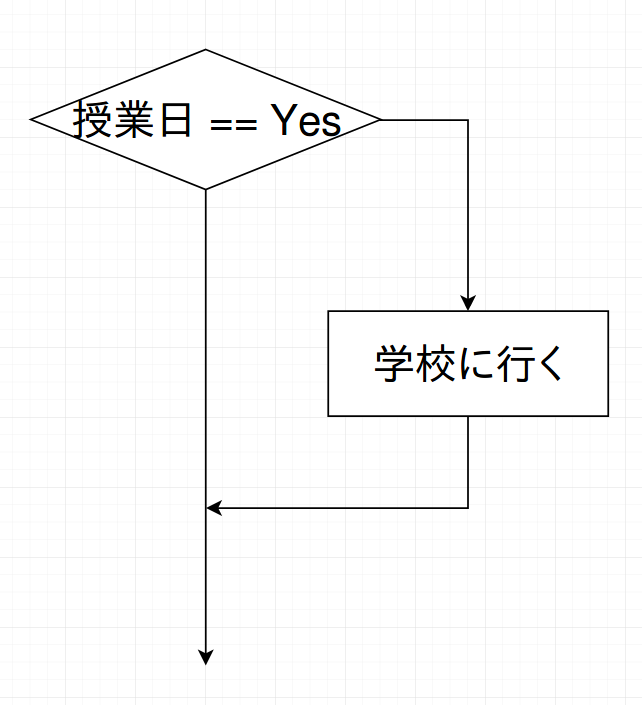
\includegraphics[width=40mm]{./choose.png}
 \end{center}
  \caption{選択}
 \end{minipage}
 \begin{minipage}{0.3\hsize}
 \begin{center}
  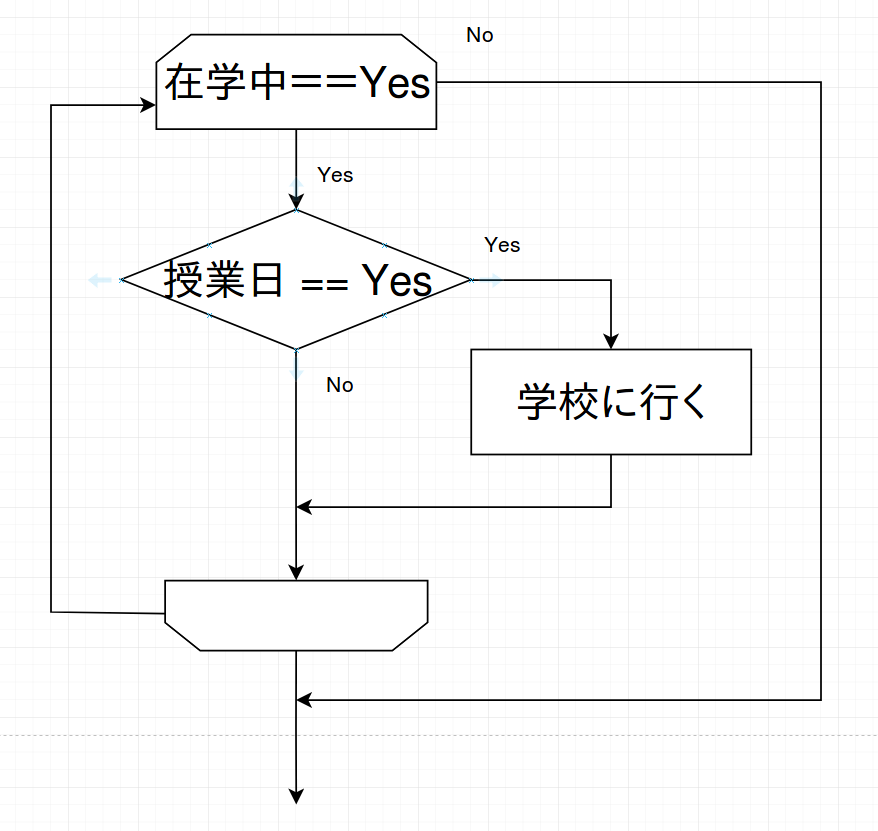
\includegraphics[width=40mm]{./repetition.png}
 \end{center}
  \caption{繰り返し}
 \end{minipage}
\end{figure}


\subsection{Pythonの基礎要素}
Pythonでプログラミングする際の基礎要素を解説します。Python2.7で実行するのを前提にしますが、Python3系で実行しても問題はないでしょう。
また、構文など多少の差異はありますが、C言語やJava、その他言語でも同じような感じです。


\newpage
\subsection{マウスを動かそう1}
このセクションでは、以下の知識を前提とします(参考サイト参照)。
\begin{lstlisting}[frame=single]
[構文]Hello world!(print文)
\end{lstlisting}

\subsubsection{サンプルプログラムの解説}
\begin{itemize}
\item{}
1〜25行目、46〜最終行は、設定のようなものなので無視してください。
\item{}
print("書きたい文字列")と書くとTerminal上に表示されます。
プログラムのどこが実行されているかを知りたい時に使うと良いでしょう。
\item{}
マウスを移動・回転させる時には、\verb|mouse.move()|を使います。構文は以下の通りです。
また、速度・回転速度制限があり、直進速度は 1[m/s] 、回転速度は π /2 [rad/s] が限界です。
ROSは右手系なので、正で半時計回りに回転します。
\end{itemize}

\begin{lstlisting}[frame=single]
mouse.move( 直進速度 [m/s], 回転速度 [rad/s])
\end{lstlisting}

\lstinputlisting[caption=micro\_mouse/script/chapter/1/moving\_mouse.py,label=moveing_mouse,numbers=left]{./../../script/chapters/1/moving_mouse.py}

\subsubsection{サンプルプログラムの実行結果}
実行結果は図\ref{moving_mouse_result}のようになります。
\begin{figure}[h]
  \begin{center}
    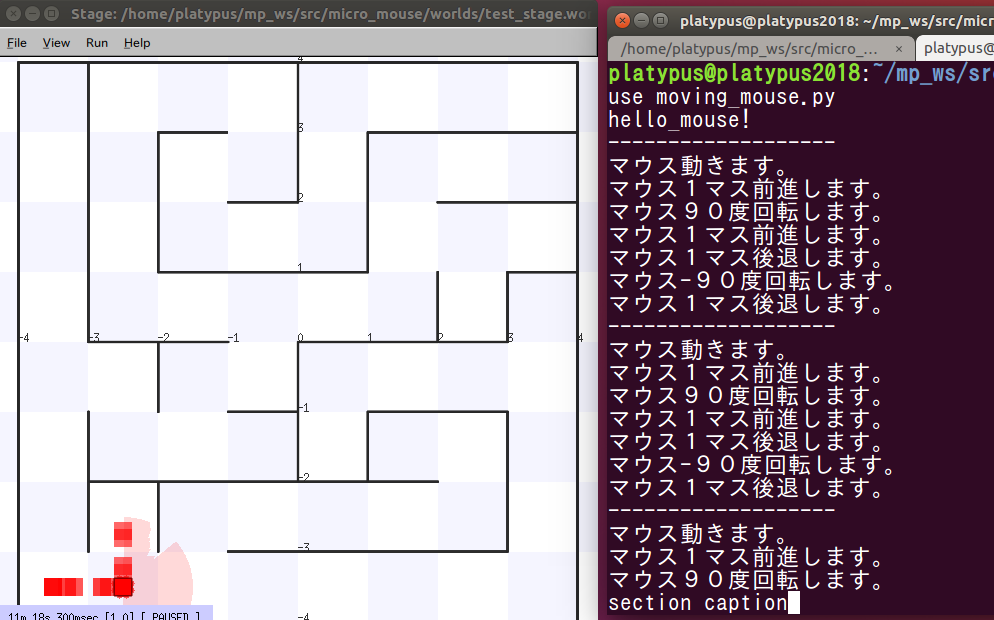
\includegraphics[width=128mm]{./moving_mouse_result.png}
  \end{center}
  \label{moving_mouse_result}
  \caption{moving\_mouse\_resultの実行結果}
\end{figure}

\subsubsection{課題}
マウスをゴール(右上)まで進ませよう。


\newpage
\subsection{マウスを動かそう2}
このセクションでは、以下の知識を前提とします(参考サイト参照)。
\begin{lstlisting}[frame=single]
[構文]Hello world! <print文>
[リスト・タプル・辞書]リスト(list)
[制御構文]もし~ならば(if, else, elsif)
[制御構文]~のあいだ(for, in)
[制御構文]ループを抜ける(break)
\end{lstlisting}

\subsubsection{サンプルプログラムの解説}
\begin{itemize}
\item{}
22〜24行目に注目してください。ここでは変数を宣言、代入しています。
pythonは変数宣言が必要ありませんが、このPDFでは一応明示的に宣言していきます。
\item{}
22行目ではリスト(配列変数)を初期化しています。
\item{}
23,24行目は使う変数を初期化しています。
\item{}
33〜43行目に注目してください。
ここではマウスのプログラムを書いています。
\item{}
33行目に注目してください。
for文でaction\_listの各要素をactionに代入しながら、
34〜42行目を繰り返しています。
\item{}
34〜41行目に注目してください。
if文でactionの数に応じて、vlとvrの値を変えています。
\item{}
42行目に注目してください。
\verb|mouse.move(vl, vr)|と書く事により、vl,vrによる制御を行っています。
つまり、for文でaction\_listから要素を1つ読み込み、それに応じて動作を行うという事を繰り返しています。
\item{}
マウスを動かそう1では、
マウスを指定の位置に移動させる場合、かなりの行数を書かなければなりませんでした。
これだと比較的短いコード量・労力で済みんじゃないでしょうか。
また、センサ値によってvl,vrを変えるようなプログラムを作れば自動化も出来そうです。
\end{itemize}

\lstinputlisting[caption=micro\_mouse/script/chapter/1/going\_mouse.py,label=going_mouse,numbers=left]{./../../script/chapters/1/going_mouse.py}

\subsubsection{サンプルプログラムの実行結果}
実行結果は図\ref{going_mouse_result}のようになります。
\begin{figure}[h]
  \begin{center}
    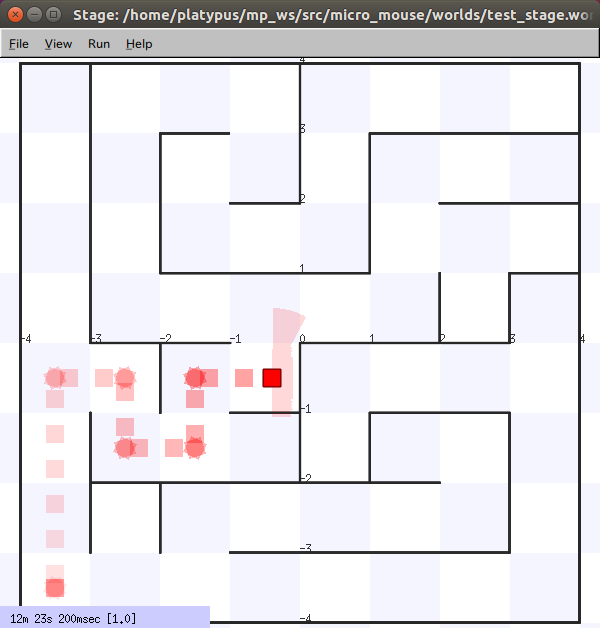
\includegraphics[width=50mm]{./going_mouse_result.png}
  \end{center}
  \label{going_mouse_result}
  \caption{going\_mouse\_resultの実行結果}
\end{figure}

\subsubsection{課題}
マウスをゴール(右上)まで進ませよう。
1つ前のセクションよりも、ずっと楽なはずです。


\newpage
\subsection{マウスのセンサを扱おう}
このセクションでは、以下の知識を前提とします(参考サイト参照)。
\begin{lstlisting}[frame=single]
[構文]Hello world! <print文>
[リスト・タプル・辞書]リスト(list)
[制御構文]もし~ならば(if, else, elsif)
[制御構文]~のあいだ(for, in)
\end{lstlisting}

\subsubsection{サンプルプログラムの解説}
\begin{itemize}
\item{}
25行目に注目してください。センサのための変数を定義しています。\\
このように書くと、[0, 0, 0, 0, 0]というような変数を確保できます。
\item{}
36行目に注目してください。mouse.sensorという配列変数にそれぞれの距離センサ値[m]が格納されています。
右辺式では、センサ値が1.0[m]以下かを判定しています
1.0[m]未満ならTrue( 1)、1.0[m]以上ならFalse( 0)が帰ってくるので、
以降、壁があるなら1、無いなら0、と簡単に考えることが出来ます。
\item{}
40,43行目に注目してください。sensor[2]==0 (壁がない)時と、else(壁がある無い、ではない時)で処理を書いています。
\end{itemize}

\begin{lstlisting}[frame=single]
mouse.sensor[ <管理番号> ]
管理番号は18〜22行目を参考にしてください。
L:左、R:右、F:前、FL:左前, FR:右前 です
\end{lstlisting}

\lstinputlisting[caption=micro\_mouse/script/chapter/1/sensing\_mouse.py,label=sensing_mouse,numbers=left]{./../../script/chapters/1/sensing_mouse.py}

\subsubsection{サンプルプログラムの実行結果}
実行結果は図\ref{sensing_mouse_result}のようになります。
\begin{figure}[h]
  \begin{center}
    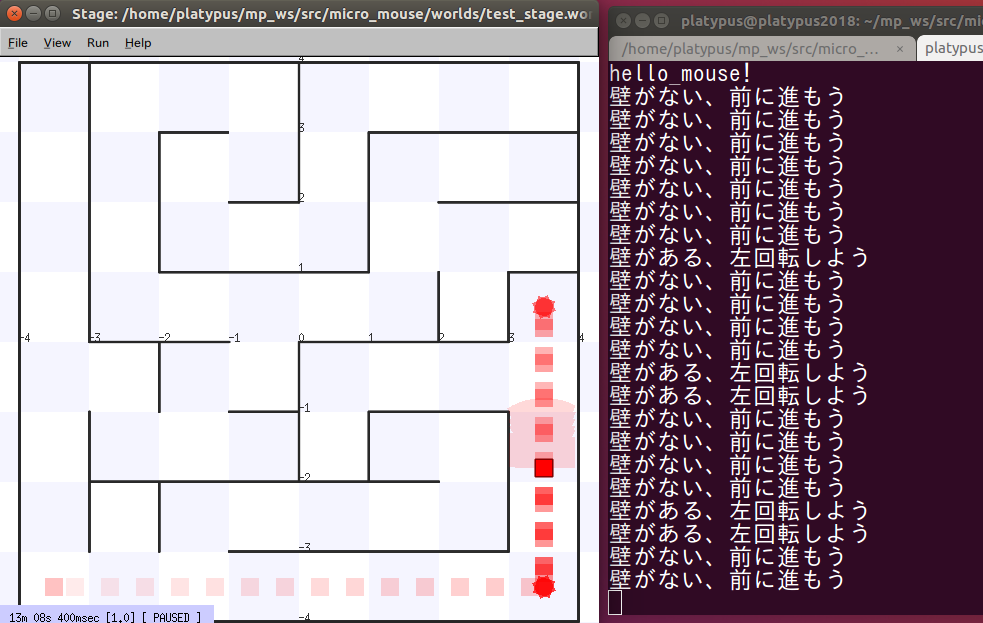
\includegraphics[width=100mm]{./sensing_mouse_result.png}
  \end{center}
  \label{sensing_mouse_result}
  \caption{sensing\_mouse\_resultの実行結果}
\end{figure}

\subsubsection{課題}
左に壁がない時、右に壁がない時を検知しよう(print等で)



\newpage
\subsection{左手法で探索しよう}
このセクションでは、以下の知識を前提とします(参考サイト参照)。
\begin{lstlisting}[frame=single]
[リスト・タプル・辞書]リスト(list)
[制御構文]もし~ならば(if, else, elsif)
[制御構文]~のあいだ(for, in)
\end{lstlisting}

\subsubsection{サンプルプログラムの解説}
特にありません。今までのセクションを参考にしてください。
\lstinputlisting[caption=micro\_mouse/script/chapter/1/left\_sensing\_mouse.py,label=left_sensing_mouse,numbers=left]{./../../script/chapters/1/left_sensing_mouse.py}

\subsubsection{サンプルプログラムの実行結果}
実行結果は図\ref{left_sensing_mouse_result}のようになります。
\begin{figure}[h]
  \begin{center}
    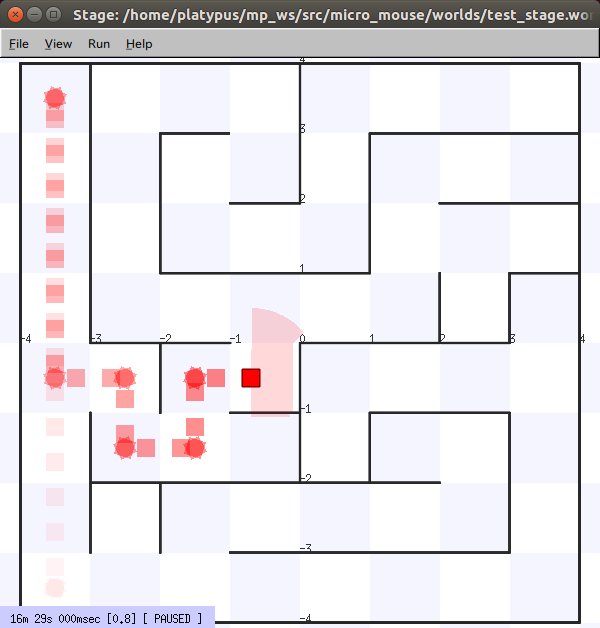
\includegraphics[width=64mm]{./left_sensing_mouse_result.png}
  \end{center}
  \label{left_sensing_mouse_result}
  \caption{left\_sensing\_mouse\_resultの実行結果}
\end{figure}

\subsubsection{課題}
右手法も作ってみよう。
また、左・右手法には欠陥があります(ある壁配置だとで全探索が出来ない)。考えよう


\newpage
\subsection{wallPublisherを使いこなそう}
\lstinputlisting[caption=micro\_mouse/script/chapter/2/wall\_publisher.py,label=wall_publisher,numbers=left]{./../../script/chapters/2/wall_publisher.py}




\newpage
\subsection{pathPublisherを使いこなそう}




\newpage
\subsection{左手法・拡張左手法・足立法を理解しよう}
\subsubsection{左手法}
\lstinputlisting[caption=micro\_mouse/script/chapter/3/left\_hund.py,label=left_hund,numbers=left]{./../../script/chapters/3/left_hund.py}


\newpage
\subsubsection{拡張左手法}
\lstinputlisting[caption=micro\_mouse/script/chapter/3/left\_hund\_ex.py,label=left_hund_ex,numbers=left]{./../../script/chapters/3/left_hund_ex.py}


\subsubsection{足立法}





\newpage
\subsection{経路計画を理解しよう}



%\lstinputlisting[caption=moving\_mouse.py,label=moveing_mouse,numbers=left]{./../script/chapters/1/moving_mouse.py}


\begin{thebibliography}{99}
\end{thebibliography}%
%
\end{document}
